\documentclass[11pt]{exam}

\usepackage{amssymb, amsmath, amsthm, mathrsfs, multicol, graphicx}
\usepackage{tikz, pgfplots}


\def\d{\displaystyle}
\def\?{\reflectbox{?}}
\def\b#1{\mathbf{#1}}
\def\f#1{\mathfrak #1}
\def\c#1{\mathcal #1}
\def\s#1{\mathscr #1}
\def\r#1{\mathrm{#1}}
\def\N{\mathbb N}
\def\Z{\mathbb Z}
\def\Q{\mathbb Q}
\def\R{\mathbb R}
\def\C{\mathbb C}
\def\F{\mathbb F}
\def\A{\mathbb A}
\def\X{\mathbb X}
\def\E{\mathbb E}
\def\O{\mathbb O}
\def\pow{\mathscr P}
\def\inv{^{-1}}
\def\nrml{\triangleleft}
\def\st{:}
\def\~{\widetilde}
\def\rem{\mathcal R}
\def\iff{\leftrightarrow}
\def\Iff{\Leftrightarrow}
\def\and{\wedge}
\def\And{\bigwedge}
\def\AAnd{\d\bigwedge\mkern-18 mu\bigwedge}
\def\Vee{\bigvee}
\def\VVee{\d\Vee\mkern-18 mu\Vee}
\def\imp{\rightarrow}
\def\Imp{\Rightarrow}
\def\Fi{\Leftarrow}



\def\circleA{(-.5,0) circle (1)}
\def\circleAlabel{(-1.5,.6) node[above]{$A$}}
\def\circleB{(.5,0) circle (1)}
\def\circleBlabel{(1.5,.6) node[above]{$B$}}
\def\circleC{(0,-1) circle (1)}
\def\circleClabel{(.5,-2) node[right]{$C$}}
\def\twosetbox{(-2,-1.5) rectangle (2,1.5)}
\def\threesetbox{(-2,-2.5) rectangle (2,1.5)}


\def\bar{\overline}

%\pointname{pts}
\pointsinmargin
\marginpointname{pts}
\marginbonuspointname{ bns pts}

\addpoints
\pagestyle{headandfoot}
%\printanswers


\header{MATH 131}{\bf\large Learning Target 2 Quiz}{Spring 2026}
\runningfooter{}{}{Version \version}
\extrafootheight{-.45 in}



\begin{document}
\def\version{A}
%space for name
\noindent {\large\bf Name:} \underline{\hspace{2.5 in}}
\vskip 1em




\begin{questions}
  \question The graph of the function $f$ is given below.  

  \begin{center}
    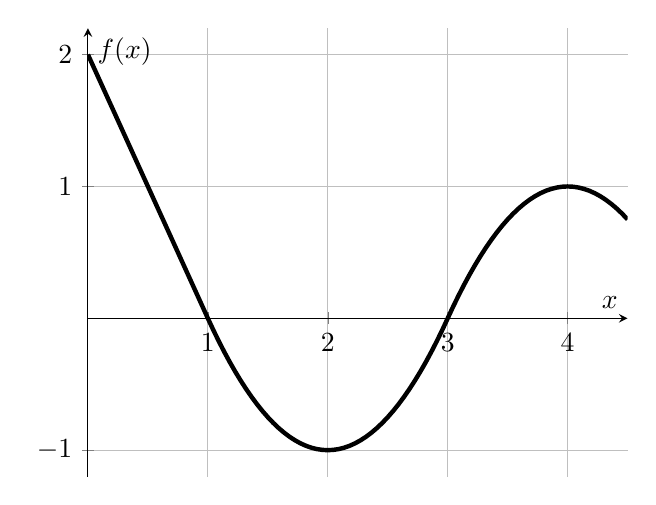
\begin{tikzpicture}[
      declare function={
        func(\x)= ( \x < 1) * (-2*\x + 2) + and(\x >= 1, \x < 3) * ((\x - 2)^2 - 1) + (\x >= 3) * (-(\x - 4)^2 + 1);
      }
    ]
      \begin{axis}[
        axis x line=middle, axis y line=middle, ymin=-1.2, ymax=2.2, xlabel=$x$, ylabel=$f(x)$, grid=major
      ]
        \addplot [domain=0:4.5,samples=100, ultra thick]{func(x)};
      \end{axis}
    \end{tikzpicture}
  \end{center}


  \begin{parts}
    \part Use the graph to find $f'(1)$, the derivative of $f$ at $a=1$.  Show your work or explain why your answer is correct.
    \vfill
    \part Where is the derivative of $f$ zero?  That is, find a value of $a$ such that $f'(a)=0$.  Explain why your answer is correct.
    \vfill
  \end{parts}


\end{questions}



\newpage

\def\version{B}
%space for name
\noindent {\large\bf Name:} \underline{\hspace{2.5 in}}
\vskip 1em




\begin{questions}
  \question The graph of the function $f$ is given below.  

  \begin{center}
    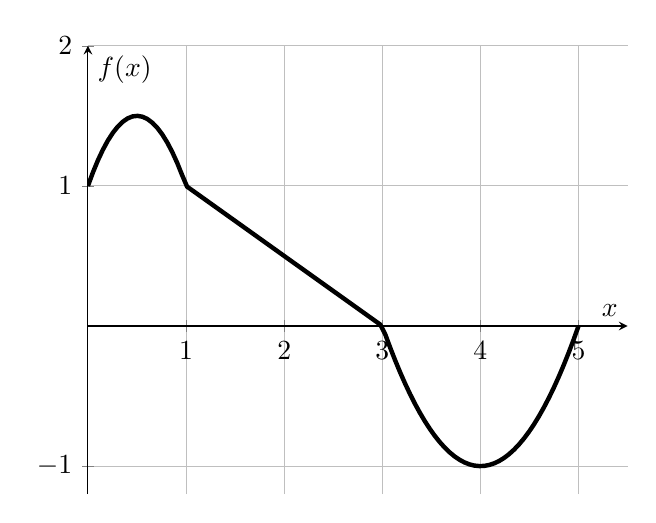
\begin{tikzpicture}[
      declare function={
        func(\x)= ( \x < 1) * (-2*(\x-0.5)^2 + 1.5) + and(\x >= 1, \x < 3) * (-0.5*\x + 1.5) + (\x >= 3) * ((\x - 4)^2 - 1);
      }
    ]
      \begin{axis}[
        axis x line=middle, axis y line=middle, ymin=-1.2, ymax=2, xmax=5.5, xlabel=$x$, ylabel=$f(x)$, grid=major
      ]
        \addplot [domain=0:5,samples=100, ultra thick]{func(x)};
      \end{axis}
    \end{tikzpicture}
  \end{center}


  \begin{parts}
    \part Use the graph to find $f'(2)$, the derivative of $f$ at $a=2$.  Show your work or explain why your answer is correct.
    \vfill
    \part Where is the derivative of $f$ zero?  That is, find a value of $a$ such that $f'(a)=0$.  Explain why your answer is correct.
    \vfill
  \end{parts}


\end{questions}

\newpage

\def\version{C}
%space for name
\noindent {\large\bf Name:} \underline{\hspace{2.5 in}}
\vskip 1em

\begin{questions}
  \question The graph of the function $f$ is given below.  

  \begin{center}
    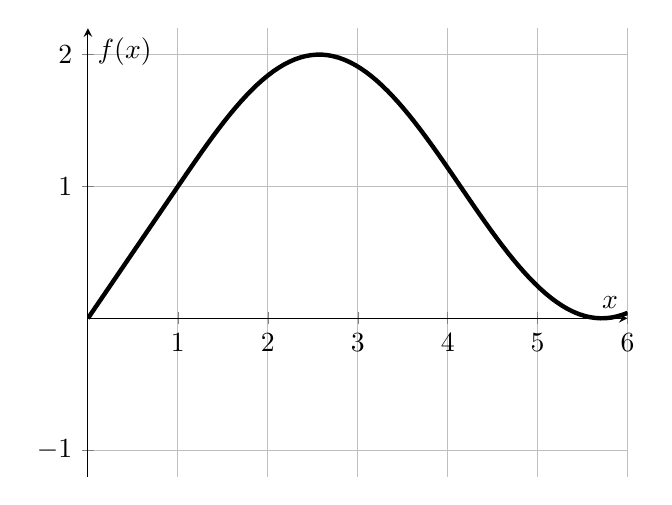
\begin{tikzpicture}[
      declare function={
        func(\x)= ( \x < 1) * (\x) + and(\x >= 1, \x < 6) * (sin(deg(\x-1)) + 1 );
      }
    ]
      \begin{axis}[
        axis x line=middle, axis y line=middle, ymin=-1.2, ymax=2.2, xlabel=$x$, ylabel=$f(x)$, grid=major
      ]
        \addplot [domain=0:6,samples=100, ultra thick]{func(x)};
      \end{axis}
    \end{tikzpicture}
  \end{center}


  \begin{parts}
    \part Use the graph to find $f'(1)$, the derivative of $f$ at $a=1$.  Show your work or explain why your answer is correct.
    \vfill
    \part Where is the derivative of $f$ zero?  That is, find a value of $a$ such that $f'(a)=0$.  Explain why your answer is correct.
    \vfill
  \end{parts}


\end{questions}


\newpage

\def\version{D}
%space for name
\noindent {\large\bf Name:} \underline{\hspace{2.5 in}}
\vskip 1em




\begin{questions}
  \question The graph of the function $f$ is given below.  

  \begin{center}
    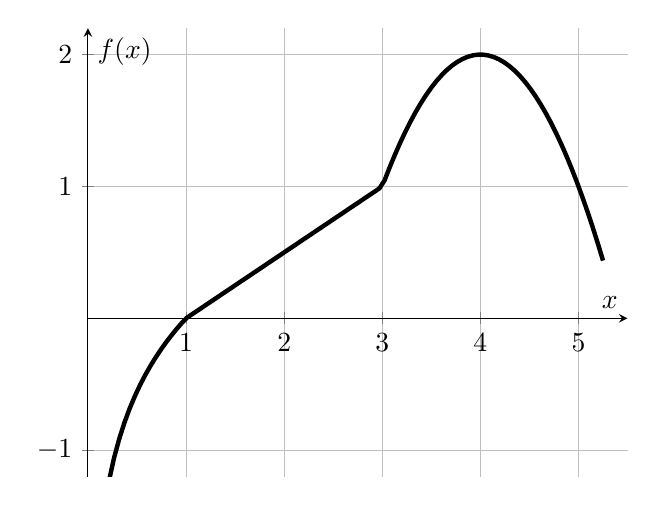
\begin{tikzpicture}[
      declare function={
        func(\x)= ( \x < 1) * (.8*ln(x)) + and(\x >= 1, \x < 3) * (0.5*\x-0.5) + (\x >= 3) * (-(\x - 4)^2 + 2);
      }
    ]
      \begin{axis}[
        axis x line=middle, axis y line=middle, ymin=-1.2, ymax=2.2, xmin=0, xmax=5.5, xlabel=$x$, ylabel=$f(x)$, grid=major
      ]
        \addplot [domain=0:5.25,samples=100, ultra thick]{func(x)};
      \end{axis}
    \end{tikzpicture}
  \end{center}


  \begin{parts}
    \part Use the graph to find $f'(2)$, the derivative of $f$ at $a=2$.  Show your work or explain why your answer is correct.
    \vfill
    \part Where is the derivative of $f$ negative?  That is, find a value of $a$ such that $f'(a) < 0$.  Explain why your answer is correct.
    \vfill
  \end{parts}


\end{questions}

\newpage

\def\version{C}
%space for name
\noindent {\large\bf Name:} \underline{\hspace{2.5 in}}
\vskip 1em

\begin{questions}
  \question The graph of the function $f$ is given below.  

  \begin{center}
    \begin{tikzpicture}[
      declare function={
        func(\x)= (\x < 3) * (4*\x-(\x)^2) + and(\x >= 3) * (9 - 2*\x);
      }
    ]
      \begin{axis}[
        axis x line=middle, axis y line=middle, ymin=-, ymax=4, xlabel=$x$, ylabel=$f(x)$, grid=major
      ]
        \addplot [domain=0:5.5,samples=100, ultra thick]{func(x)};
      \end{axis}
    \end{tikzpicture}
  \end{center}


  \begin{parts}
    \part Use the graph to find $f'(4)$, the derivative of $f$ at $a=1$.  Show your work or explain why your answer is correct.
    \vfill
    \part Where is the derivative of $f$ zero?  That is, find a value of $a$ such that $f'(a)=0$.  Explain why your answer is correct.
    \vfill
  \end{parts}


\end{questions}



\end{document}
